% !TeX spellcheck = de_DE
\section{Optimierungsprobleme}
\label{sec:analysis_optimzation_problems}
Nach erfolgreicher Verifizierung der Funktionalität wird in diesem Kapitel auf verschiedene andere Optimierungsprobleme eingegangen, anhand derer die Analyse durchgeführt werden soll. Grundsätzlich ist bei der Implementierung zu beachten, dass keine zu aufwendigen Optimierungsprobleme verwendet werden, da der Raspberry Pi 4 nicht so leistungsfähig ist und die benötigte Optimierungszeit sehr hoch sein kann. Daher werden im Folgenden hauptsächlich klassische Probleme des bestärkenden Lernens aus dem OpenAI Gym verwendet. Die ausgewählten Umgebungen sind das \emph{Cartpole}, \emph{MountainCar} und \emph{Pendulum} Problem. Im Folgenden wird auf die entsprechenden Optimierungsprobleme genauer eingegangen und die Implementierung der Fitnessfunktion und Abbruchbedingung vorgestellt. 

\subsection{Cartpole}
Die \emph{Cartpole} Umgebung, auch als \emph{Pole Balancing} bezeichnet, wurde bereits 1983 in Quelle \cite{barto1983neuronlike} vorgestellt und ist auch heute noch ein bekanntes Optimierungsproblem, welches in vielen Publikationen verwendet wird. Auch im OpenAI Gym ist dieses Problem entsprechend der Beschreibung aus Quelle \cite{barto1983neuronlike} enthalten und in Abbildung \ref{fig:cartpole_environment} dargestellt. In der Umgebung befinden sich zwei Gegenstände, ein Wagen und ein Balken. Der Wagen kann vom Agenten nach links und rechts bewegt werden. Hierauf befindet sich der Balken, der am unteren Ende mit dem Wagen verbunden ist und entsprechend seiner Position nach links oder rechts kippen kann. Ziel des Agenten ist, durch Steuerung des Wagens den Balken so lange wie möglich senkrecht zu balancieren. Bezüglich der Abbruchbedingung gilt, dass der Agent scheitert, wenn  sich der Balken um mehr als 15 Grad zur Seite neigt oder der Wagen zu weit vom Zentrum entfernt ist. Als Eingabewerte für das \ac{KNN} werden von der Umgebung vier Werte zur Verfügung gestellt, für welche je ein Eingabeneuron erstellt wird. Dies ist unter anderem die Position und Geschwindigkeit des Wagens, der aktuelle Winkel des Balkens und dessen Änderungsrate. Zusätzlich besitzt das erstellte \ac{KNN} zwei Ausgabeneuronen, welche die jeweilige Richtung repräsentieren. Ist der Aktivierungsgrad des erstens \emph{Output}-Neurons höher als der des zweiten, wird der Wagen nach links bewegt und andernfalls nach rechts.
\begin{figure}[!h]
	\centering
	
\includegraphics[width=0.5\textwidth]{./img/cartpole_env.JPG} 
	\caption{Darstellung der \emph{Cartpole} Umgebung aus dem OpenAI Gym}
	\label{fig:cartpole_environment}
\end{figure} 
Bevor die Evaluation mit dieser Umgebung durchgeführt wird, müssen die Fitnessfunktion, Lösungsbedingung und Konfiguration festgelegt werden. Beim klassischen bestärkenden Lernen, wie in Kapitel \ref{subsubsec:reinforcment_learning} beschrieben, erhält der Agent nach jedem Zeitschritt einen \emph{reward}. Da das OpenAI Gym primär für diese Art des Lernens konzipiert ist, wird auch hier nach jeder Aktion in der Umgebung ein \emph{reward} zurückgegeben. In diesem Fall erhält ein Agent bis zum Scheitern für jeden Zeitschritt einen \emph{reward} mit der Wertigkeit $1$. Mit diesen muss für neuroevolutionäre Algorithmen eine Fitnessfunktion definiert werden. Bei diesem Beispiel ist das Vorgehen einfach. Der Fitnesswert wird berechnet, indem die erhaltenen \emph{rewards} aggregiert und der resultierende Wert am Ende der Evaluation quadriert wird. Somit soll wie zuvor beim XOR-Problem besseren Agenten ein proportional höherer Fitnesswert zugewiesen werden. Das Optimierungsverfahren wird beendet, wenn ein Agent den Balken 500 Zeitschritte balancieren kann. Die restlichen Parameter wurden aus dem vorherigen Beispiel übernommen und nicht geändert.
\begin{figure}[!h]
	\centering
	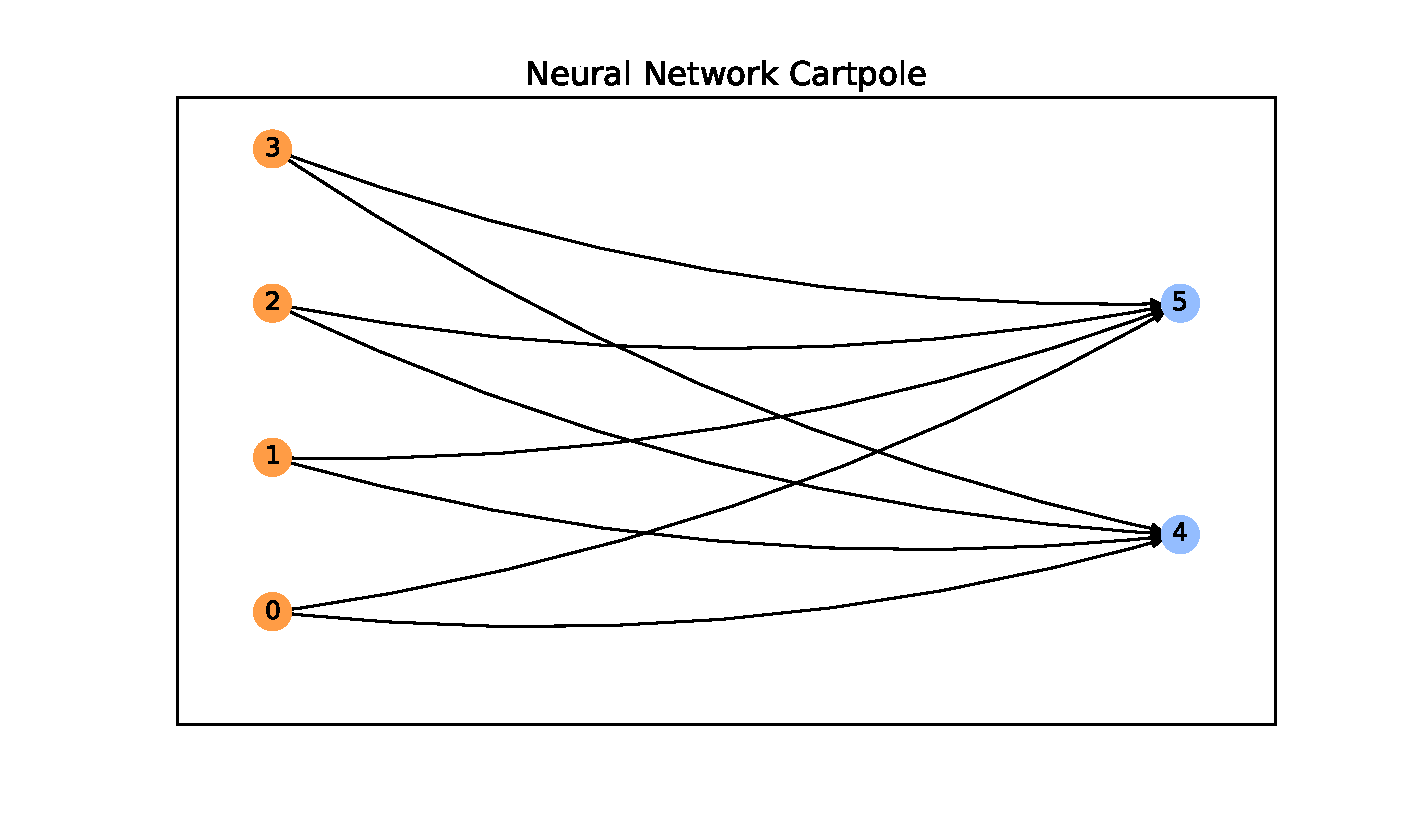
\includegraphics[width=0.7\textwidth]{./img/pole_balancing_single_core/cartpole_neuroal_network.pdf} 
	\caption{Struktur des finalen KNN im \emph{Cartpole} Optimierungsproblem}
	\label{fig:cartpole_neural_network}
\end{figure}
\\\\
Allerdings stellt sich beim Ausführen dieses Optimierungsproblems heraus, dass es für die Analyse ungeeignet ist. Bereits bei den zufällig erstellten Agenten der initialen Population sind \ac{KNN} vorhanden, welche die Abbruchbedingung erfüllen und das Optimierungsproblem lösen. Ein solches ist in Abbildung \ref{fig:cartpole_neural_network} dargestellt. Wie die anderen \ac{KNN} in der initialen Population besitzt auch dieses keine \emph{Hidden}-Neuronen und zeigt, dass für das Lösen dieses Optimierungsproblems keine komplexen Entscheidungen notwendig sind. Es ist beispielsweise möglich, mit dem Winkel des Balkens auf die auszuführende Aktion zu schließen. Neigt sich der Balken nach rechts, bewegt sich der Wagen in diese Richtung und umgekehrt. Dies ist einer der Gründe, warum dieses Optimierungsproblem im weiteren Verlauf der Arbeit nicht weiter verwendet wird. Ein weiterer Grund ist, dass aufgrund der fehlenden Optimierung keine Ausführungszeiten über mehrere Generationen gemessen werden können, welche eine notwendige Grundlage für den späteren Vergleich sind.

\subsection{Mountain Car}
\label{subsec:analysis_mountain_car}
Die Umgebung \emph{Mountain Car} ist ein weiteres Optimierungsproblem, welches aus dem OpenAI Gym stammt und in Abbildung \ref{fig:mountain_car_env} dargestellt ist. Das Ziel für den Agenten ist, den Wagen auf den rechten Berg zu fahren, wo sich eine Fahne befindet. Hierfür stehen ihm Steuerungsoptionen für den Antrieb des Wagens zur Verfügung. Bei jedem Zeitschritt kann der Agent entscheiden, ob er nach links, rechts oder gar nicht beschleunigen möchte. Die Schwierigkeit dabei ist, dass der Antrieb nicht stark genug ist, um den Wagen direkt zum Ziel auf der rechten Bergspitze zu fahren. Das Ziel kann nur erreicht werden, wenn der Wagen zunächst ein Stück den linken Berg hochfährt, in einer gewissen Höhe die Richtung wechselt und beschleunigt. Mit dem zusätzlichen Schwung kann der Wagen dann die rechte Bergspitze erreichen. Für dieses Optimierungsproblem gibt es zwei Eingabewerte. Der erste ist die aktuelle Position des Wagens, der zweite seine Geschwindigkeit. Auf Basis von diesen muss der Agent seine Aktion wählen. Auch für diese Umgebung muss eine Abbruchbedingung und Fitnessfunktion festgelegt werden. Die Ausführung der Umgebung wird beendet, wenn der Agent entweder das Ziel auf der rechten Seite erreicht oder $200$ Zeitschritte vergangen sind. Allerdings ist das Erreichen der Fahne allein nicht ausreichend, um das \emph{Mountain Car} Problem erfolgreich zu lösen. Laut der Dokumentation des OpenAI Gyms muss der Agent dies in $100$ aufeinander folgenden Evaluationen in durchschnittlich $110$ Zeitschritten oder weniger schaffen.
\begin{figure}[!h]
	\centering
	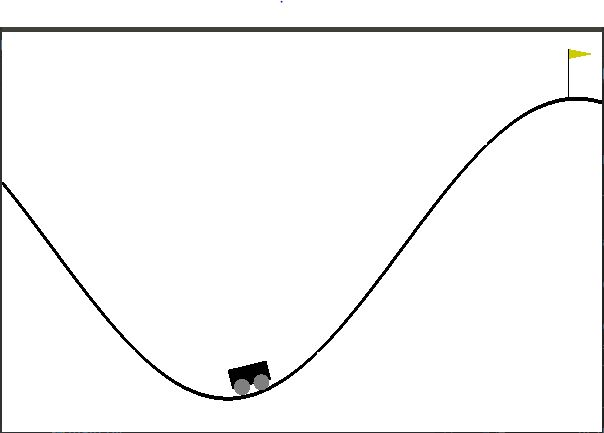
\includegraphics[width=0.5\textwidth]{./img/mountain_car_env.JPG} 
	\caption{Darstellung der \emph{Mountain Car} Umgebung aus dem OpenAI Gym}
	\label{fig:mountain_car_env}
\end{figure} 
\\\\
Grundsätzlich kann dies implementiert werden, indem beispielsweise nach jeder Generation der beste Agent $100$ mal in verschiedenen Umgebungen getestet wird. Aber da dies die Trainingszeit stark erhöhen würde und die Laufzeit auf dem Raspberry Pi 4 vergleichsweise hoch ist, wird eine einfachere Bedingung gewählt. Das Trainingsverfahren wird beendet, wenn es einem Agenten erstmalig gelingt, das \emph{Mountain Car} Problem in weniger als $110$ Zeitschritten erfolgreich zu beenden. Zuletzt muss die Fitnessfunktion implementiert werden. Die \emph{Mountain Car} Umgebung gibt für jeden Zeitschritt einen \emph{reward} von $-1$. Für eine bessere Übersichtlichkeit und zur Vermeidung negativer Fitnesswerte wird dieser auf den Wert $200$ initialisiert. Für jeden benötigten Zeitschritt wird ein Punkt abgezogen. Bessere Agenten, die weniger Zeitschritte benötigten, erhalten so einen höheren Fitnesswert. Allerdings kann es vorkommen, dass kein Agent der initialen Population das Ziel auf der rechten Seite erreicht. In diesem Fall würde jeder Agent den Fitnesswert $0$ haben, wodurch keine Selektion möglich ist. Aus diesem Grund wird die maximal erreichte X-Koordinate ebenfalls in den Fitnesswert miteinbezogen. Sollte kein Agent das Ziel erreichen, haben die Agenten, welche diesem am nächsten waren, einen Selektionsvorteil. Zuletzt wird der Fitnesswert wie auch zuvor quadriert, um besseren Agenten einen proportional höheren Fitnesswert zuzuweisen. Die restliche Konfiguration für diese Umgebung ist ähnlich zu den vorherigen Beispielen. Einzig die Populationsgröße wird auf $300$ Agenten erhöht, da dieses Problem aufwendiger zu lösen ist als die vorherigen.
\\\\
Prinzipiell kann das Verfahren ab diesem Punkt evaluiert werden, allerdings varieren die maximalen Fitnesswerte in vielen Fällen stark. Der Grund hierfür ist eine verrauschte Fitnessfunktion, wie es in Kapitel \ref{subsec:comparision_neuroevoltion} erläutert ist. Die Startposition des Wagens ist zufällig durch die Umgebung gesetzt und kann einen großen Einfluss auf den Fitnesswert haben. So kann es vorkommen, dass ein Agent einen hohen Fitnesswert aufgrund einer günstigen Startposition erhält, ansonsten aber schlechte Ergebnisse erzielen würde. Ein Ansatz zur Minimierung dieses Effektes besteht darin, dass jeder Agent mehrfach die Evaluation durchführen muss und der mittlere Fitnesswert verwendet wird. Ein Vorteil dabei ist, dass der Agent mit verschiedenen Situationen konfrontiert wird und somit die Eigenschaft der Generalisierung erfüllt. Ein Nachteil ist, dass dadurch die Trainingszeit stark erhöht wird. Der Fokus in dieser Arbeit liegt auf dem Vergleich zwischen der sequenziellen und parallelisierten Implementierung. Da dafür die Eigenschaft der Generalisierung nicht notwendig ist, wird ein anderer Ansatz gewählt. Die Umgebungen werden so konfiguriert, dass jeder Agent mit derselben Ausgangssituation beginnt, wodurch sich die Trainingszeiten verringern und ein Vergleich einfacher umzusetzen ist.
\begin{figure}[!h]
	\centering
	\begin{minipage}[]{0.49\textwidth}
		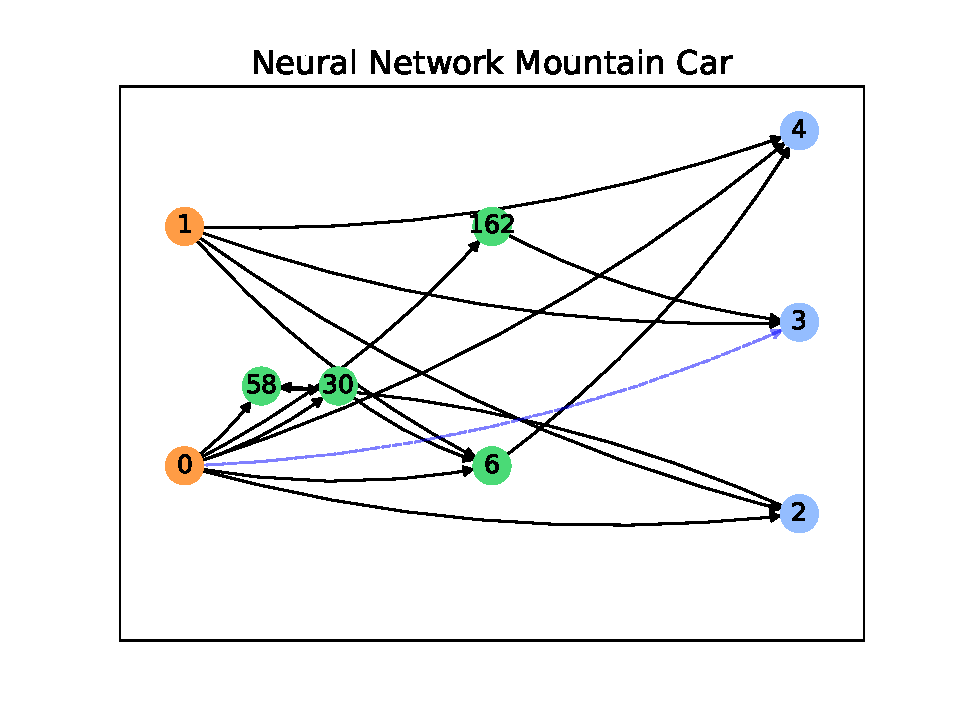
\includegraphics[width=1.0\textwidth]{./img/mountain_car_single/mountain_car_neural_network.pdf} 
	\end{minipage}
	\hfill
	\begin{minipage}[]{0.49\textwidth}
		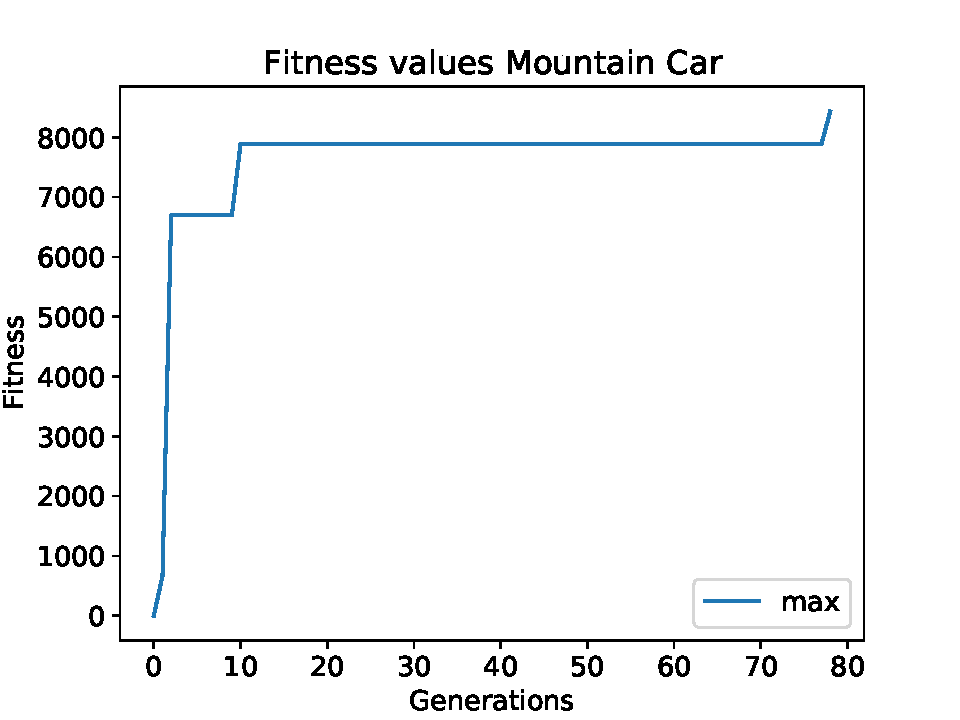
\includegraphics[width=1.0\textwidth]{./img/mountain_car_single/1413_fitness_1core_1pi.pdf} 
	\end{minipage}
	\caption{Links die Lösung für das Mountain Car Problem, rechts die dazugehörigen Fitnesswerte pro Generation}
	\label{fig:mountain_car_1core_neural_network_and_fitness}
\end{figure}
\\\\
Mit der vorgestellten Konfiguration wird das Optimierungsproblem durchgeführt. Die Ergebnisse sind in Abbildung \ref{fig:mountain_car_1core_neural_network_and_fitness} und \ref{fig:mountain_car_time_single_core} dargestellt. Das \ac{KNN} links in Abbildung \ref{fig:mountain_car_1core_neural_network_and_fitness} enthält vier \emph{Hidden}-Neuronen. Zusätzlich sind sowohl zyklische als auch deaktivierte Verbindungen enthalten. In der Abbildung rechts ist der maximale Fitnesswert dargestellt. Innerhalb der ersten $10$ Generationen steigt dieser schnell auf $7888$ an, da der Agent $113$ Zeitschritte zum Lösen gebraucht hat. Da für das erfolgreiche Lösen nicht mehr als $110$ Zeitschritte genutzt werden dürfen, versucht der Algorithmus eine bessere Lösung zu finden. Allerdings stagniert der Fortschritt bis Generation $78$, in der eine bessere Lösung gefunden wird, welche die Abbruchbedingung erfüllt. Abbildung \ref{fig:mountain_car_time_single_core} zeigt die benötigte Ausführungszeit für diesen Versuch. Insgesamt wurden ungefähr $105$ Minuten für das Trainingsverfahren benötigt. Aus der Abbildung ist erkennbar, dass diese Zeit maßgeblich durch die \emph{Evaluation Time} bestimmt ist. Insgesamt wurden $98\%$ der Ausführungszeit für die Evaluation der Agenten verwendet. Die restlichen zwei Prozent teilen sich die \emph{Compose Offspring Time} und \emph{Reproduction Time}. Letztere hat mit insgesamt ca. $9$ Sekunden die geringste Ausführungszeit benötigt. Für die Rekombination und Mutation von Agenten wurden insgesamt $113$ Sekunden verwendet. Bezüglich der gesamten Ausführungszeit ist festzustellen, dass diese für jede Generation tendenziell ansteigt, auch wenn es einzelne Spitzen oder Einbrüche gibt. Hierfür kann es verschiedene Gründe geben. Die Ausführungszeit wird einerseits von der Größe der \ac{KNN} beeinflusst, welche im Laufe des Verfahrens größer werden. Die Einbrüche in der Ausführungszeit können beispielsweise entstehen, wenn die Agenten großteils das Ziel früh erreichen und somit weniger Zeitschritte simuliert werden müssen. Alternativ kann die Ausführungszeit sinken, wenn große \ac{KNN} schlechte Fitnesswerte erzielt haben und daher nicht für die Reproduktion ausgewählt werden.  
\begin{figure}[!h]
	\centering
	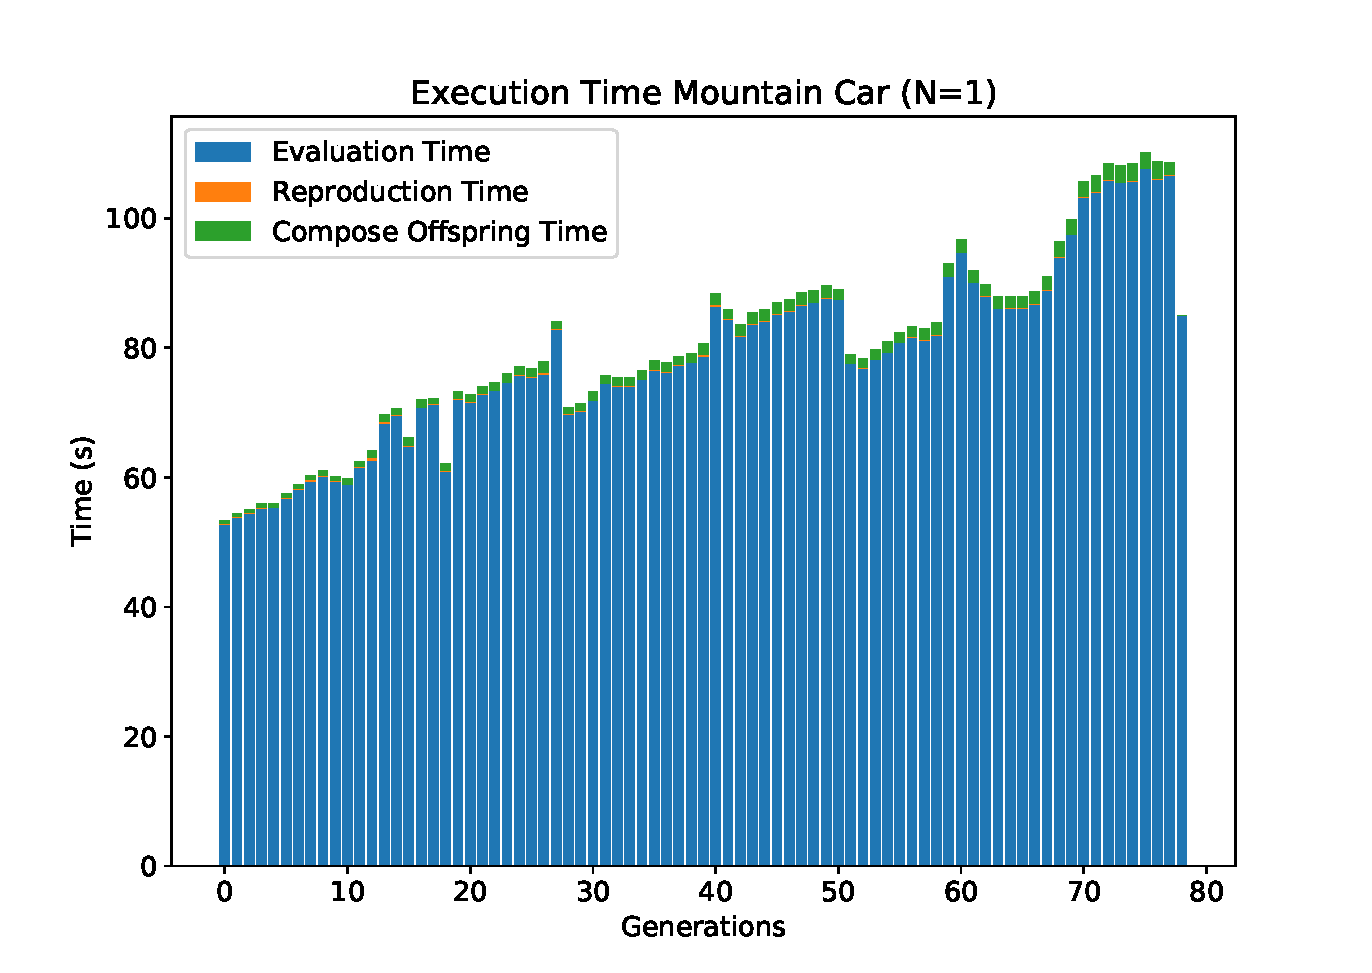
\includegraphics[width=0.7\textwidth]{./img/mountain_car_single/1413_time_1core_1pi.pdf} 
	\caption{Ausführungszeiten des Mountain Car Problems auf einem Raspberry Pi 4 mit einem Prozess}
	\label{fig:mountain_car_time_single_core}
\end{figure}% TODO Maybe regenerate Graph? Text of axis has a different size

\subsection{Pendulum}
\label{subsec:analysis_pendulum}
\begin{figure}[!h]
	\centering
	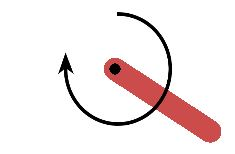
\includegraphics[width=0.3\textwidth]{./img/pendulum_env.JPG} 
	\caption{Darstellung der \emph{Pendulum} Umgebung aus dem OpenAI Gym}
	\label{fig:pendulum_env}
\end{figure}
\noindent
Die letzte Umgebung, welche im Rahmen der Analyse betrachtet wird, ist das \emph{Pendulum} aus dem OpenAI Gym, welches in Abbildung \ref{fig:pendulum_env} dargestellt ist. In der Umgebung befindet sich ein Pendel mit einer initial zufälligen Position und Geschwindigkeit. Die Aufgabe des Agenten ist, dieses in eine senkrechte Position zu bringen und dort so lang wie möglich zu halten. Hierfür stehen ihm drei Eingabewerte zur Verfügung, von denen zwei die aktuellen Winkel des Pendels und der dritte die Bewegungsgeschwindigkeit repräsentieren. Entsprechend besitzt das \ac{KNN} drei Eingabeneuronen, auf Basis derer eine Aktion ausgewählt wird. Der Agent kann prinzipiell Kraft nach links oder rechts ausüben, um das Pendel zu bewegen. Allerdings gibt es einen Unterschied zu den vorherigen Testumgebungen. Bei diesen kann der Agent nur die Richtung entscheiden, in welche eine konstante Kraft wirken soll. Dies sind diskrete Entscheidungsprobleme. In dieser Umgebung muss der Agent nicht nur die Richtung, sondern auch die auszuübende Kraft bestimmen. Das bedeutet konkret für diese Umgebung, dass ein Wert zwischen $-2$ und $2$ gewählt werden muss. Ist der Wert negativ, wird die Kraft nach links ausgeübt, andernfalls nach rechts. Die auszuübende Kraft wird durch die absolute Größe des Wertes bestimmt. Das \ac{KNN} erhält einen Ausgabewert und verwendet die \ac{tanh} Funktion für die Aktivierung, welche Werte zwischen $-1$ und $1$ zurückgibt. Um die auszuführende Kraft zu berechnen, wird der Ausgabewert vor dem Ausführen der Aktion mit $2$ multipliziert. Die Fitnessfunktion für diese Umgebung besteht wieder aus der Aggregation der einzelnen \emph{rewards}, welche durch das OpenAI Gym für jeden Zeitschritt gegeben werden. Ein einzelner \emph{reward} kann zwischen $\approx -16.2$ und $0$ liegen. Dies ist abhängig von der aktuellen Position und Geschwindigkeit des Pendels sowie der ausgeübten Kraft. Das Ziel ist, mit möglichst wenig Kraftaufwand das Pendel aufrecht zu halten. Das Trainingsverfahren wird beendet, wenn ein Agent einen Fitnesswert von $-200$ erreicht. Bezüglich der sonstigen Konfiguration ist anzumerken, dass bei diesem Optimierungsproblem keine zyklischen Verbindungen zugelassen werden und die Populationsgröße auf $1000$ Agenten erhöht ist. Im Zuge dessen wird auch die Kompatibilitätsfunktion mit den Werten $c_3=4.0$ und $\delta_t=3.5$ angepasst. Das Ziel dieser Änderung ist, dass den Gewichtsunterschieden eine höhere Priorität zugewiesen wird und unterschiedliche Strategien entwickelt werden können. Zuletzt ist bezüglich der Umgebung anzumerken, dass der Startzustand bei diesem Optimierungsproblem aus den selben Gründen wie in Kapitel \ref{subsec:analysis_mountain_car} beschrieben für alle Agenten gleich ist.  
\begin{figure}[!h]
	\centering
	\begin{minipage}[]{0.49\textwidth}
		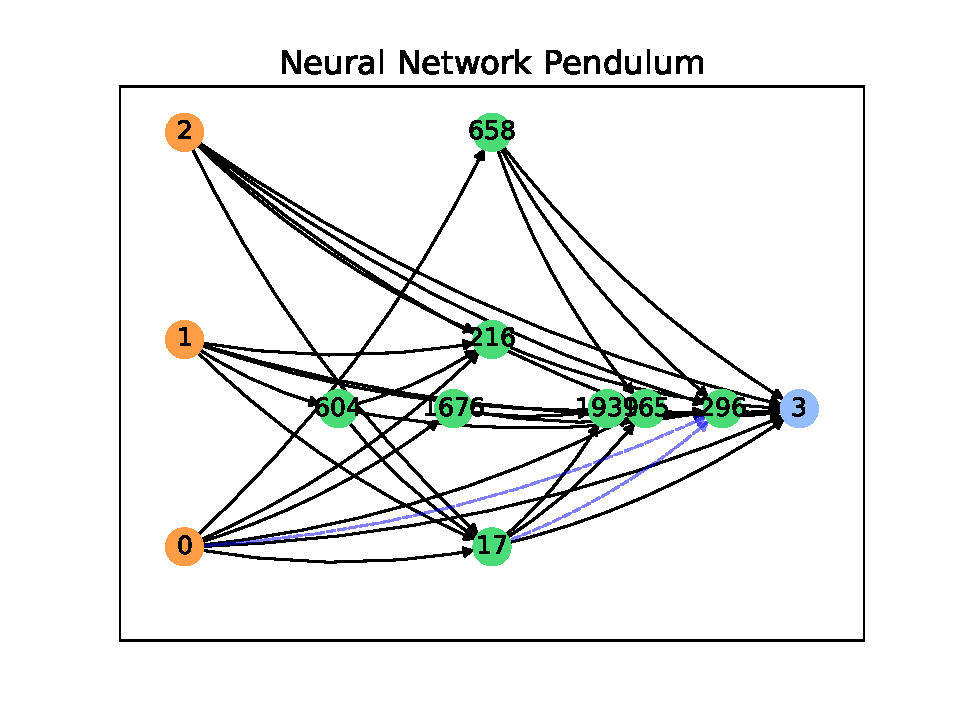
\includegraphics[width=1.0\textwidth]{./img/pendulum_single_core/pendulum_1_neural_network.pdf} 
	\end{minipage}
	\hfill
	\begin{minipage}[]{0.49\textwidth}
		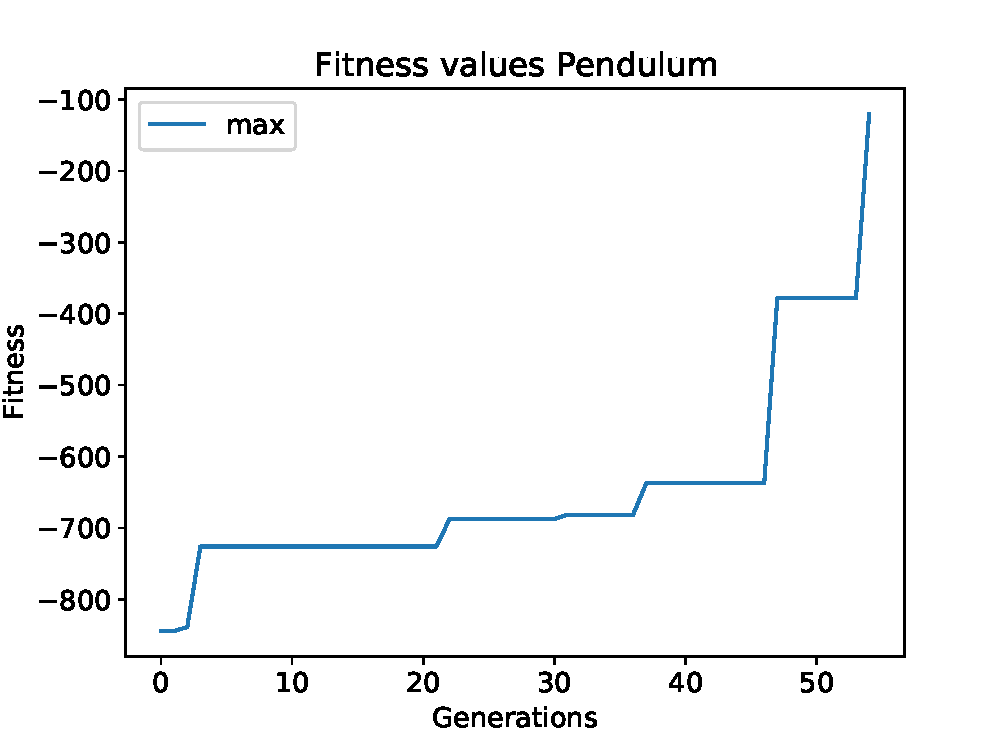
\includegraphics[width=1.0\textwidth]{./img/pendulum_single_core/pendulum_1_fitness_values.pdf} 
	\end{minipage}
	\caption{Links die Lösung für das Pendulum Problem, rechts die dazugehörigen Fitnesswerte pro Generation}
	\label{fig:pendulum_car_1core_neural_network_and_fitness}
\end{figure}
\\\\
Das Verfahren wird mit der spezifizierten Konfiguration durchgeführt, die erhaltenen Ergebnisse sind in Abbildung \ref{fig:pendulum_car_1core_neural_network_and_fitness} und \ref{fig:pendulum_1core_1pi_time} dargestellt. Insgesamt hat der Algorithmus 55 Generationen evaluiert und einen finalen Fitnesswert von ca. $-120$ erreicht. Mit dem dargestellten \ac{KNN} hat der Agent in der letzten Evaluation das Pendel beim ersten Versuch aufgerichtet und während der restlichen Simulation ausbalanciert. Bezüglich der Fitnesswerte zu erkennen, dass der Agent zwar immer wieder Fortschritte erzielt, aber auch einige Generationen lang stagniert. Dies ist ähnlich zu den vorherigen Beispielen. Die Ausführungszeiten hingegen haben sich etwas geändert. Insgesamt hat die Evaluation $125.8$ Minuten gedauert. Wie zuvor beim \emph{Mountain Car} Problem ist die Ausführungszeit während des Verfahrens stetig gestiegen. Allerdings gibt es im Gegensatz zum vorherigen Beispiel keine großen Einbrüche. Ein möglicher Grund hierfür ist, dass die Umgebung immer $200$ Zeitschritte ausgeführt wird, unabhängig von der Leistung des Agenten bzw. seinem \ac{KNN}. Mit insgesamt $91\%$ Anteil hat die \emph{Evaluation Time} den größten Einfluss auf die Ausführungszeit. Die \emph{Compose Offspring Time} hat bei diesem Durchlauf insgesamt $180$ Sekunden und damit nur etwa $2\%$ der Ausführungszeit benötigt. Die restlichen $7\%$ werden für die \emph{Reproduction Time} genutzt, welche insgesamt ungefähr $574$ Sekunden angedauert hat. Der Grund hierfür ist, dass durch die veränderte Kompatibilitätsfunktion bedeutend mehr Spezies entstanden sind. Die Folge ist, dass für das Zuweisen von Nachkommen für jede Spezies und vor allem für das Sortieren der Agenten in diese bedeutend mehr Rechenaufwand entsteht. 

\begin{figure}[!h]
	\centering
	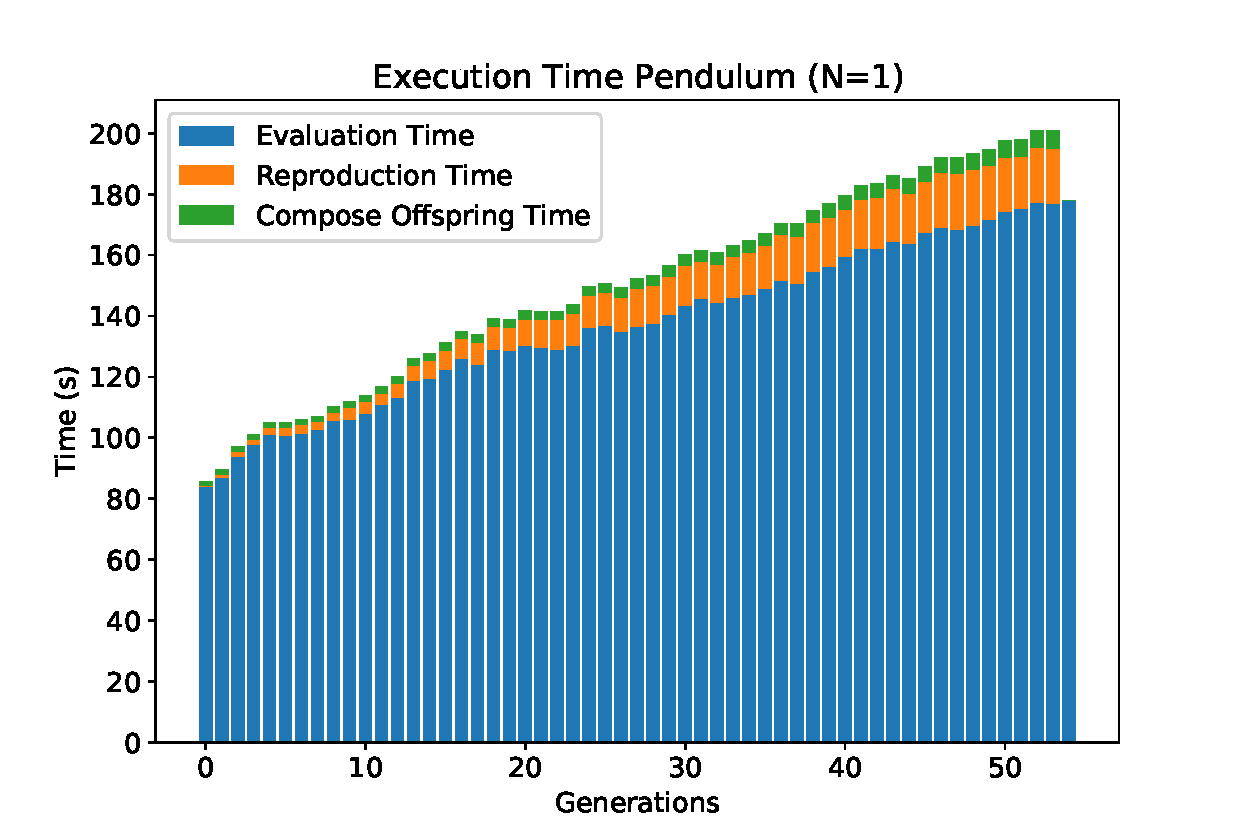
\includegraphics[width=0.7\textwidth]{./img/pendulum_single_core/pendulum_1_1core_1pi_time.pdf} 
	\caption{Ausführungszeiten des Pendulum Problems auf einem Raspberry Pi 4 mit einem Prozess}
	\label{fig:pendulum_1core_1pi_time}
\end{figure}


